\begin{frame}\frametitle{Performing Localisation in Real Missions}
\begin{block}{Rectangular trajectory in low depth}
\begin{columns}
\column{.78\textwidth}
Fairly noisy GPS signal (antenna is on the surface) was used as position correction. Parameters $\sigma_{north},\sigma_{east}$ of north and east measurement noise can be set (~\ref{fig:ne10}, ~\ref{fig:ne05}). Reasonably chosen values significantly correct the result obtained with pure dead reckoning. %Giving extremely high confidence with such amount of noise does not seem to be the best choice, however,
\column{.2\textwidth}
\centering
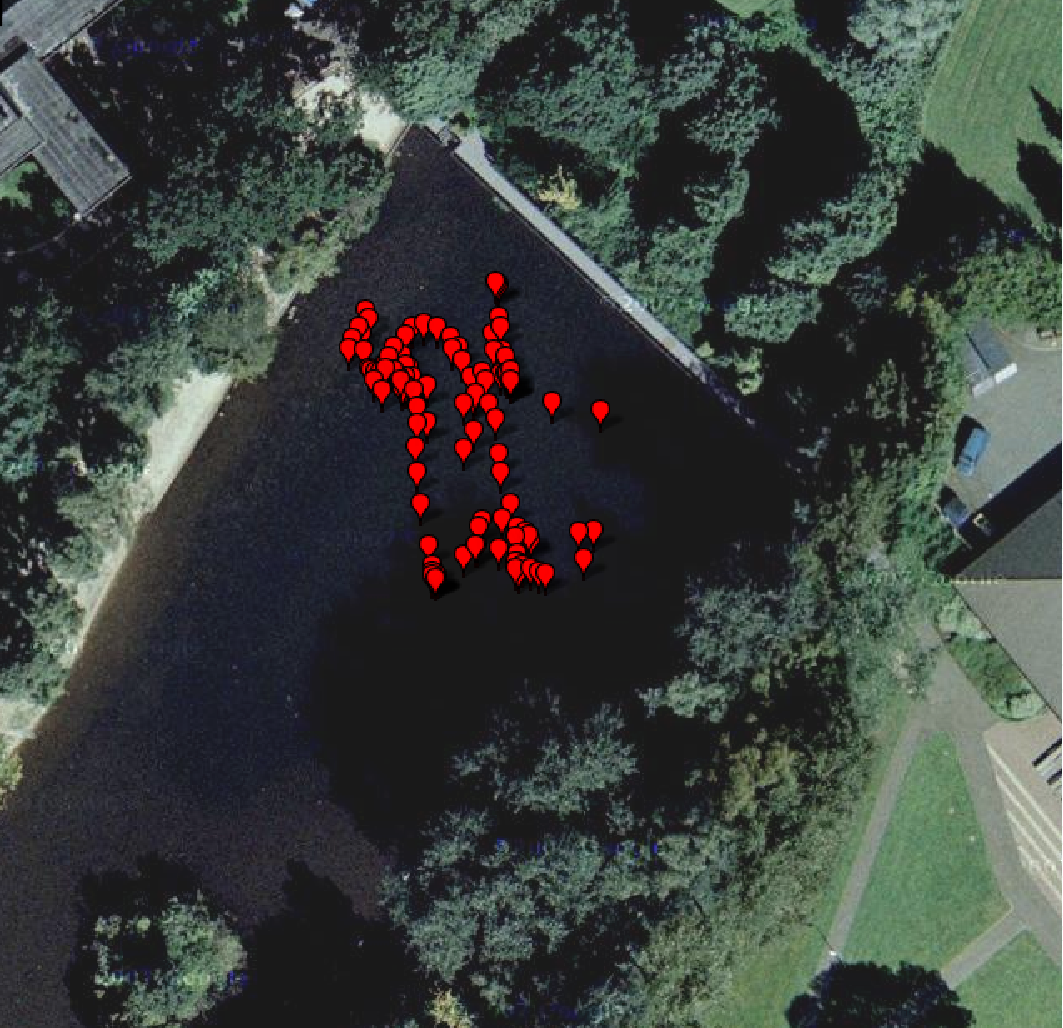
\includegraphics[width=0.95\linewidth]{fig/square-trajectory.pdf}
\end{columns}
\end{block}
\vspace{-10pt}
\centering 
\begin{figure}%(confidence in position measurement)  _{north}=\sigma_{east}  a_{north}=\sigma_{east}
\subfigure[{\scriptsize N/E localisation $\sigma= 1.0 m $}]{\label{fig:ne10} 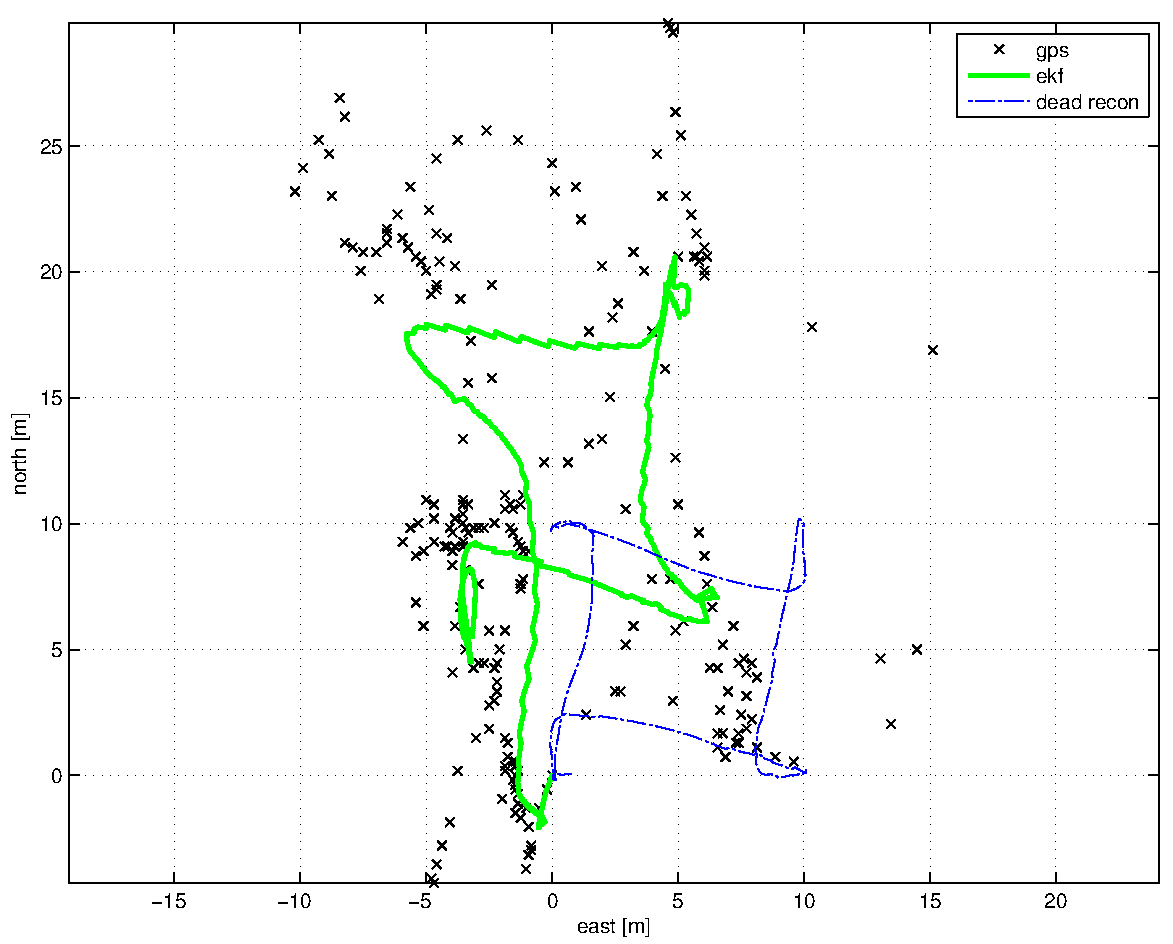
\includegraphics[width=0.32\linewidth]{fig/square10.pdf}} 
\subfigure[{\scriptsize N/E localisation $\sigma= 0.5 m $}]{\label{fig:ne05} 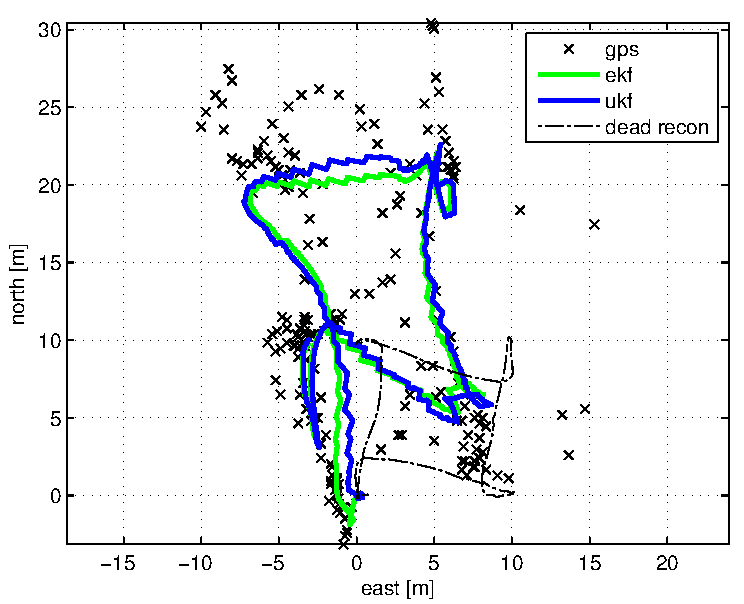
\includegraphics[width=0.32\linewidth]{fig/square05.pdf} }
\subfigure[{\scriptsize Velocities \& heading}]{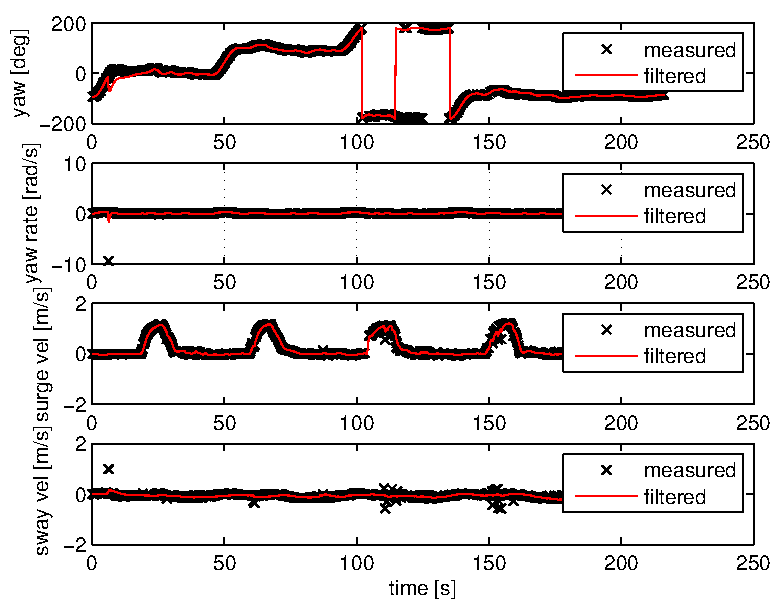
\includegraphics[width=0.3\linewidth]{fig/dynamics.pdf}}
\vspace{-10pt}
\caption{Rectangular trajectory localisation}
\vspace{-10pt}
\end{figure}
%From a noisy collection of position observations at the beginning, application of EKF with sensor fusion enabled having generally better performance in navigation.
\end{frame}